\documentclass[12pt, letterpaper]{article} 
\usepackage{amsmath, amssymb, amsthm, enumerate, graphicx, fancyhdr}
\pagestyle{fancy}

\begin{document}
\graphicspath{ {./} }

\fancyhead[L]{\textbf{Math 110 HW 5}}
\fancyhead[C]{\textbf{Spring 2026}}
\fancyhead[R]{\textbf{Dani Nguyen}}

\noindent \textbf{Question 1}
\begin{enumerate}[(a)]
    \item Given $\phi(x) = e^{-x^2},\ \psi(x) = 0$
    \begin{align*}
        u(x,t) &= \frac{1}{2}\left(e^{-(x-ct)^2 }+ e^{-(x+ct)^2}\right)+\frac{1}{2c}\int_{x-ct}^{x+ct}0ds \\
        &= \frac{1}{2}\left(e^{-(x-ct)^2 }+ e^{-(x+ct)^2}\right)
    \end{align*}
    \begin{center}
        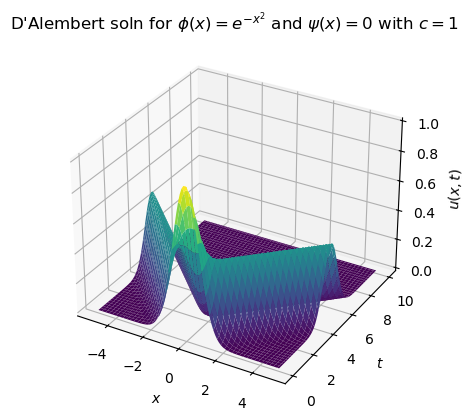
\includegraphics[scale=0.85]{1a.png}
    \end{center}
    \newpage
    \item Given $\phi(x) = 0,\ \psi(x) = \cos x$
    \begin{align*}
        u(x,t) &= \frac{1}{2}\left(0+ 0\right)+\frac{1}{2c}\int_{x-ct}^{x+ct}\cos(s)ds \\
        &= \frac{1}{2c}\Big[\sin(s)\Big]^{x+ct}_{x-ct} \\
        &= \frac{1}{2c}\Big[\sin(x+ct) - \sin(x-ct)\Big]
    \end{align*}
    \begin{center}
        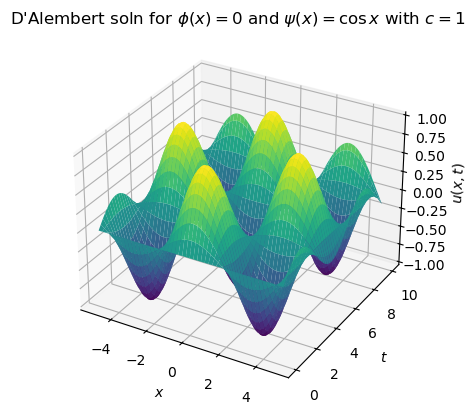
\includegraphics[scale=0.85]{1b.png}
    \end{center}
    \newpage
    \item Given $\phi(x) = \begin{cases}
        1 & |x| < 1 \\
        0 & \text{otherwise}
    \end{cases}\ ,\quad \psi(x) = 0$ \\ \\
    For $|x| < 1$,
    \begin{align*}
        u(x,t) &= \frac{1}{2}\left(1+1\right) \\
        &= 1 
    \end{align*}
    For $|x| > 1$
    \begin{align*}
        u(x,t) &= 0
    \end{align*}
    \begin{align*}
        u(x,t) &= \begin{cases}
            1 & |x| < 1 \\
            0 & \text{otherwise}
        \end{cases}
    \end{align*}
    \begin{center}
        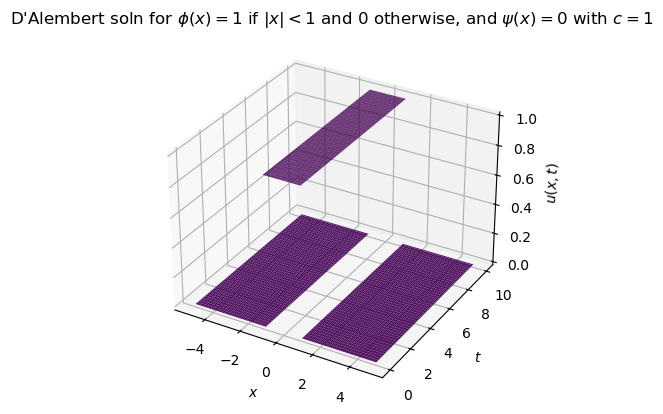
\includegraphics[scale=0.85]{1c.png}
    \end{center}
    \newpage
    \item Given $\phi(x) = 0,\ \psi(x) = e^{-|x|}$
    \begin{align*}
        u(x,t) &= \frac{1}{2c} \int_{x-ct}^{x+ct}e^{-|s|}ds \\
        &= \begin{cases}
            \frac{1}{2c} \int_{x-ct}^{x+ct}e^{s}ds & s < 0\\
            \frac{1}{2c} \int_{x-ct}^{x+ct}e^{-s}ds & s > 0\\
        \end{cases} \\
        &= \begin{cases}
            \frac{1}{2c} \Big[e^{s}\Big]_{x-ct}^{x+ct} & s < 0\\
            \frac{1}{2c} \Big[-e^{-s}\Big]_{x-ct}^{x+ct} & s > 0\\
        \end{cases} \\
        &= \begin{cases}
            \frac{1}{2c} \Big[e^{x+ct}-e^{x-ct}\Big] & \quad x < -ct\\
            \frac{1}{2c} \Big[-e^{-(x+ct)}-e^{(x-ct)}\Big] + \frac 1c& -ct < x < ct\\
            \frac{1}{2c} \Big[-e^{-(x+ct)}+e^{-(x-ct)}\Big] & \quad x > ct\\
        \end{cases} 
    \end{align*}
    \begin{center}
        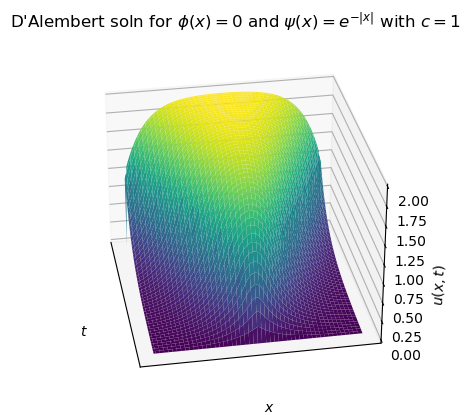
\includegraphics[scale=0.85]{1d.png}
    \end{center}
\end{enumerate}
\newpage
\noindent \textbf{Question 2}
\begin{enumerate}[(a)]
    \item 
\end{enumerate}
\noindent \textbf{Question 3} \\
\noindent \textbf{Question 4} \\
\noindent \textbf{Question 5} \\

\end{document}